
\section{The One-World Feature of Kent's Theory\label{OneWorldFeature}}
The third similarity Kent's theory shares with the Bohmian interpretation is that it is a one-world interpretation of quantum physics. It will be helpful to contrast this with the many-worlds interpretation. 

 Unlike the many-worlds interpretation, Kent's theory does not allow for indeterminate states of macroscopic objects such as cats. In the many-worlds interpretation, Schr\"{o}dinger will still only observe his cat to be either dead or alive, and not both dead and alive. However, Schr\"{o}dinger himself goes into a superposition of observing his cat to be alive and his cat to be dead. In the many-worlds interpretation, there is thus a difference between observing something to be so, and something actually being so: the observation is of a particular physical scenario, but the reality is a superposition of different physical scenarios. 

To capture this distinction between observation and reality, Bell speaks of \textbf{beables}\index{beable}.\label{beabledef} Bell introduces the term beable when speculating on what would be a more satisfactory physical theory than what quantum physics currently has to offer.\footnote{See \cite{Bell2}} Bell says that such a theory should be able to say of a system not only that such and such is observed to be so, but that such and such be so. In other words, a more satisfactory theory would be a theory of beables rather than a theory of observables. On the macroscopic level, these beables should be the underlying reality that gives rise to all the familiar things in the world around us, things like cats, laboratories, procedures, and so on. For example proponents of the Bohmian interpretation believe that the beables are all the particles each with their precise position and momentum. But whatever these beables are, it is because of them that a scientist can observe a physical system to be in such and such a state. Thus, observables are ontologically dependent on beables.   

Now the beables in Kent's one-world interpretation are expressed in terms of a physical quantity called the \textbf{stress-energy tensor}\index{stress-energy tensor}  $T^{\mu\nu}(y)$.\label{stressenergy}   %
\nomenclature{$T^{\mu\nu}(y)$}{The stress-energy tensor, \nomrefpage}%
For any spacetime location $y$, the stress-energy tensor $T^{\mu\nu}(y)$ is an array of 16 values corresponding to each combination of $\mu, \nu=0,1,2,$ or $3$. %
\nomenclature{$\mu, \nu$}{Generic indices of tensors, $\mu, \nu=0,1,2,$ or $3$, \nomrefpage}%
 The value $T^{00}(y)$ is the energy density at $y$ divided by $c^2$,\footnote{This is not to be confused with the mass-energy density $T_S(x)$ defined for $x$ on a hypersurface $S$. As will be shown in section \ref{LorentzInvariance},   all 16 elements of $T^{\mu\nu}(x)$ will typically be needed to calculate $T_S(x)$.} whereas the other values of $T^{\mu\nu}(y)$ indicate how much energy and momentum flow across different surfaces in the neighborhood of $y$. 



It was mentioned in the previous section that for any spacetime location $x\in S$,  there is an observable $\hat{T}_S(x)$ acting on $H_S$ corresponding to the mass-energy density $T_S(x)$ of the surface $S$ at $x$. It turns out that for any $\mu, \nu=0,1,2,$ or $3$, there is also an observable  $\hat{T}^{\mu\nu}(x)$ acting  %
\nomenclature{$\hat{T}^{\mu\nu}(x)$}{The observable corresponding to the stress-energy tensor $T^{\mu\nu}(y)$ in the Tomonaga-Schwinger picture, \nomrefpage}%
 on $H_S$, such that if $\ket{\Psi}\in H_S$ is a simultaneous eigenstate of $\hat{T}^{\mu\nu}(x)$ with eigenvalue $\tau^{\mu\nu}(x)$ for  %
\nomenclature{$\tau^{\mu\nu}(x)$}{For fixed $\mu,\nu$, the simultaneous eigenvalue for all $x\in S$ of a simultaneous eigenstate $\hat{T}^{\mu\nu}(x)$, \nomrefpage}%
 all $x\in S$, then $\ket{\Psi}$ corresponds to a state of $S$ in which $T^{\mu\nu}(x)$ is  $\tau^{\mu\nu}(x)$ for all $x\in S$.\footnote{Note however, that such a simultaneous eigenstate is only for a fixed choice of $\mu$ and $\nu$, since in general, $\hat{T}^{\mu\nu}(x)$ and $\hat{T}^{\mu'\nu'}(x)$ will not commute for $\mu\neq\mu'$ or $\nu\neq\nu'$. } Moreover, the observable $\hat{T}_S(x)$ is expressible in terms of the  $\hat{T}^{\mu\nu}(x)$-observables.\footnote{See section  \ref{LorentzInvariance} for an explanation for why this is so.}\textsuperscript{,}\footnote{As in (\ref{approxeigen2}), we have the same implicit understanding of $\hat{T}^{\mu\nu}(x)$ and $\tau^{\mu\nu}(x)$ as being defined over cells $c_x\subset S$ rather than at spacetime locations $x\in S$, though we will often speak of them as being defined at spacetime locations. }
Now the  beables in Kent's theory are defined at each spacetime location $y$ that occurs after $S_0$ and before $S$. For such a spacetime location $y$, the beables will be determinate values of the stress-energy tensor $T^{\mu\nu}(y)$, but calculated from the expectation of the observable $\hat{T}^{\mu\nu}(y)$ conditional on the mass-energy density $T_S(x)$ on $S$ being given by $\tau_S(x)$ for all the $x\in S$ that are outside the light cone of $y$. 

Kent implicitly assumes that a specification of the stress-energy tensor $T^{\mu\nu}(y)$ for all spacetime locations $y$ between $S_0$ and $S$ will be sufficient to give a macroscopic description of physical reality between $S_0$ and $S$.\footnote{See \cite[2]{Kent2014} where he talks about giving a description of reality between $S_0$ and $S$.} This seems like a reasonable assumption, since from the $T^{00}(y)$ component of the stress-energy tensor, we will be able to tell how much energy is present in the vicinity of $y$, and from the other components of the stress-energy tensor, we will be able to work out how much of this energy is due to mass and how much is due to motion. Thus, from the stress-energy tensor, we will be able to form a picture of where things are and whether things are equilibrium or whether there are flows of matter and energy from one region to another. Such a description of reality will also include information about measurement readings that scientists observe when performing their experiments, so although  we wouldn't expect there to be a complete specification of physical reality down to the microscopic level in terms of the stress-energy tensor, there will be enough information in the stress-energy tensor at the macroscopic level to make various scientific claims about physical reality at the microscopic level. 

In section \ref{kentcalculation}, we will come back to the question of why we can't include any information about $\tau_S(x)$ for $x\in S$ within the light cone of $y$ when we discuss how the conditional expectations of the stress-energy density are calculated. But before we do that, we first consider why we should need conditional expectations at all in order to provide a one-world description of reality.


To this end, we recall the definition of expectation in equation (\ref{expectation2}) and the expectation formula (\ref{evev}) for an observable. In a theory that posited the beables to be the expectation values of $\hat{T}^{\mu\nu}(y)$ for any $y$ located between $S_0$ and $S$  without conditioning on the value of the mass-energy density $T_S$ on $S$, then the $T^{\mu\nu}(y)$-beable would just be $\ev*{\hat{T}^{\mu\nu}(y)}{\Psi_{S'}}$ where $\ket*{\Psi_{S'}}=U_{S'S_0}\ket{\Psi_0}$ for any hypersurface $S'$ that goes through $y$.\footnote{This can be done such that $\ev*{\hat{T}^{\mu\nu}(y)}{\Psi_{S'}}$ does not depend on the hypersurface $S'$ other than the fact that it contains $y$. For more details see \cite{SchwingerJulianI}.} However, such a beable would give a description of reality that was very different from what we observe. For instance, in a Schr\"{o}dinger cat-like experiment (see section \ref{SchrondingersCat}), there would be a stress-energy tensor distribution corresponding to both the cat being alive and the cat being dead in the same world as depicted in figure \ref{deadlivecat}.
\begin{figure}[ht!]
  \captionsetup{justification=justified}
  \centering
  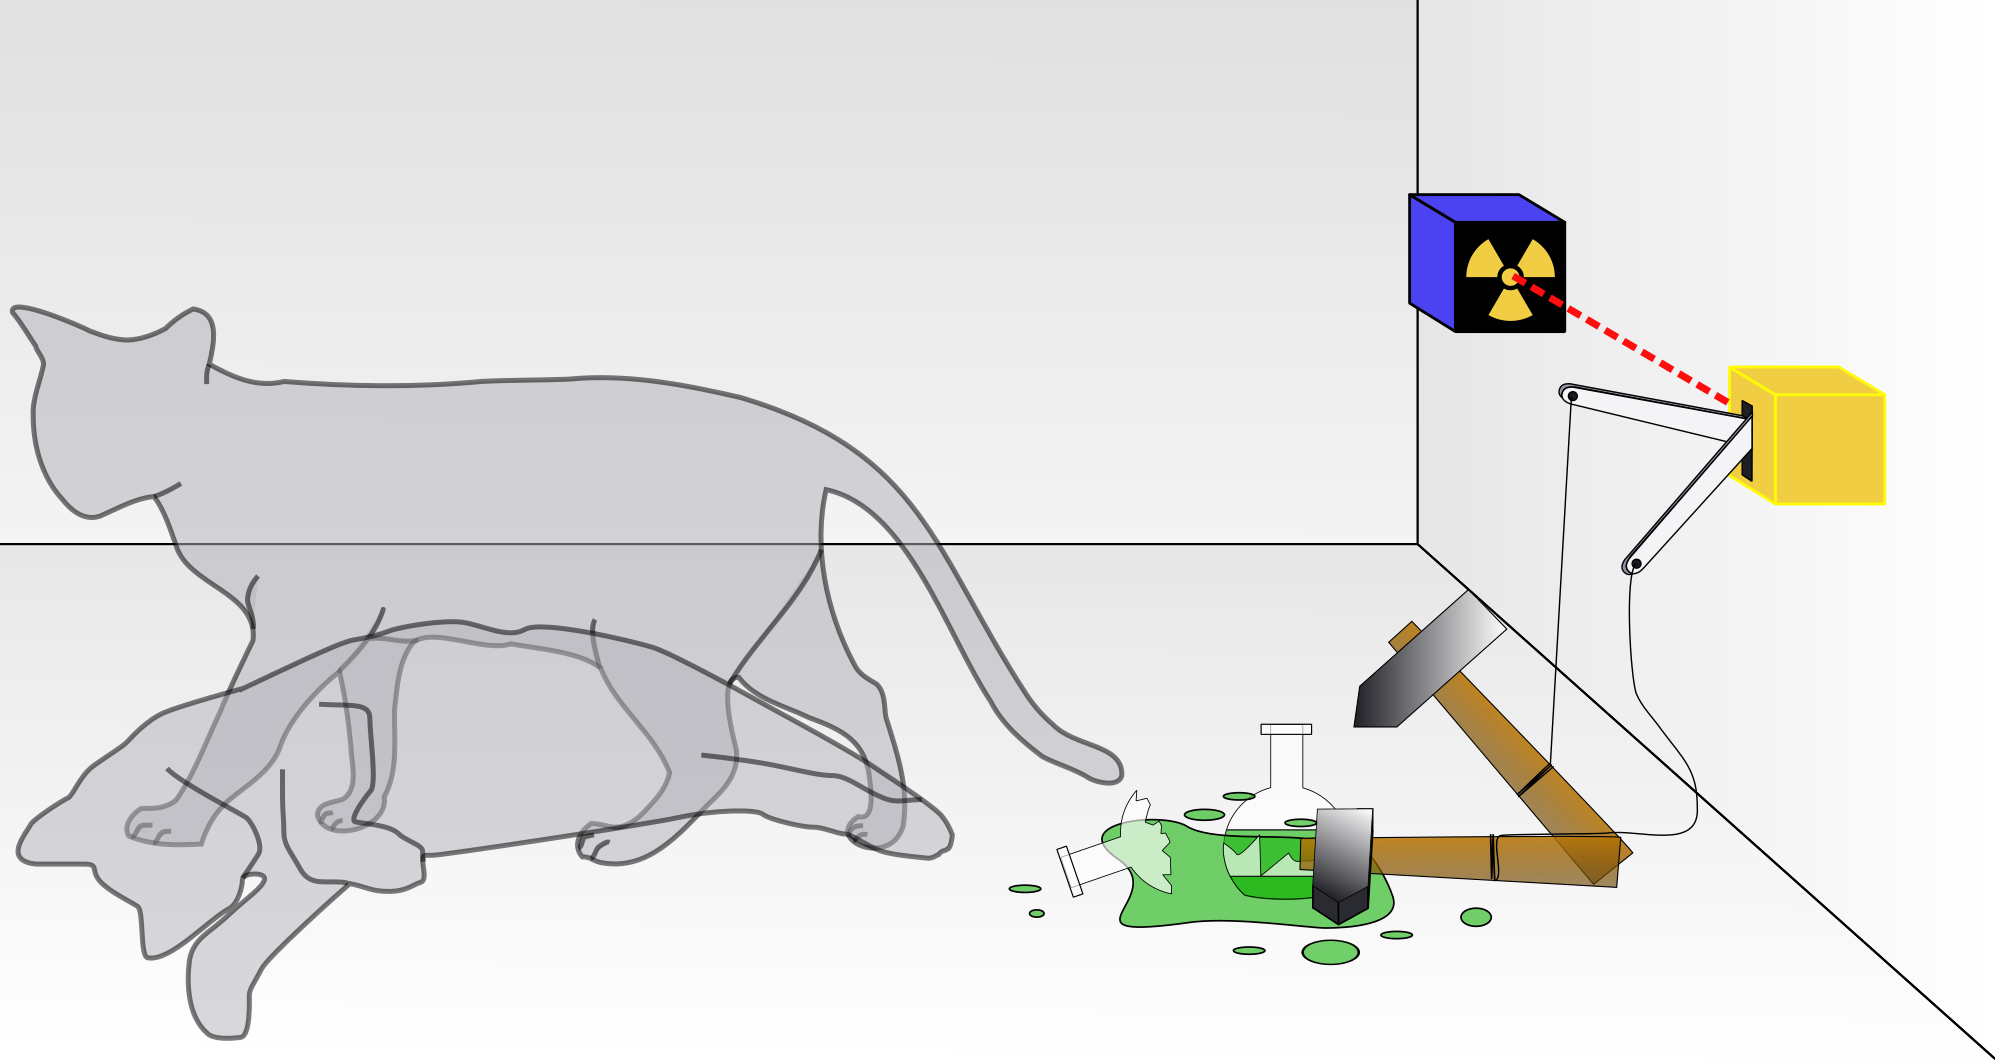
\includegraphics[width=100mm]{Chapter03/Schrodingers_cat.png}
  \caption[Depiction of Schr\"{o}dinger's cat]{A depiction of Schr\"{o}dinger's cat being both dead and alive.\protect\footnotemark}
  \label{deadlivecat}
  \end{figure}
  \footnotetext{ Original by Dhatfield. This image is licensed under the Creative Commons Attribution-Share Alike 3.0 Unported license. Source: https://commons.wikimedia.org/wiki/File:Schrodingers\_cat.svg}
  Such a distribution arises in this context because initially there is an atom that is in a superposition of decayed and non-decayed states, and so the expectation of $\hat{T}^{\mu\nu}(y)$ will have non-zero components both in the location where the non-decayed atom would be, and also in the locations of the decayed atom and the particle the atom emitted. As the decayed atom part of the state interacts with the poison releasing device, this device will also enter into a superposition so that in both the location of the poison containing flask and in the locations of all the poison atoms in the container containing the cat and into which the poison is released, the expectation of $\hat{T}^{\mu\nu}(y)$ will have non-zero components. And then the cat will enter into a superposition of being in a dead state and an alive state, and so  the expectation of $\hat{T}^{\mu\nu}(y)$ will have non-zero components in locations where the dead cat ends up and where the living cat happens to be. So the expectation of $\hat{T}^{\mu\nu}(y)$ in the locations of the container containing the cat will be very different from what someone would actually observe. To see how bizarre a description of reality would be if we just based it on unconditioned expectation values of observables, suppose we had an observable $A$ whose value was $1$ if the cat was alive and $0$ if the cat was dead, then assuming the decay probability was $1/2$, the expected value of $A$ would be $1/2$. Therefore, if we were to rely on such an expectation value in describing physical reality, we would have to say that the cat was literally half-dead and half-alive. 

  To overcome this defect, information about the mass-energy density on $S$ is used, specifically the values of $\tau_S(x)$ for $x\in S^1(y)$ where  $S^1(y)$  %
  \nomenclature{$S^1(y)$}{The set  of all the spacetime locations of $S$ outside the light cone of $y$, \nomrefpage}%
  is defined to consist of all the spacetime locations of $S$ outside the light cone of $y$ as depicted in figure \ref{S2}.  

 \begin{figure}[ht!]
\captionsetup{justification=justified}
\centering

\tikzmath{
\a= 1;  
\e = 0.1;
\h=-1;
\hae=(3*\a*\a+6*\a*\e+7*\e*\e-3*\a*sqrt(\a*\a+4*\e*\e)-4*\e*sqrt(\a*\a+4\e*\e))/(4*\a+4*\e-2*sqrt(\a*\a+4*\e*\e));
\hae=0.0463647;
\hae=0.0858615;
\circsize=1.2;
\md = (\a+\h)/2;
\lrange = 4;
\rrange=2;
\ss=(-\lrange-\a)/2;
\sss=\a+(\rrange-\a)/2;
\tlen=0.75;
\labelpos=(-\lrange-\a)/2;
} 

\begin{tikzpicture}[thick, scale=2]

\def\dotsize{0.7}

\definecolor{tempcolor}{RGB}{0,151,76}
\draw[<->] (-\lrange, \h) node[left] {$S_0$} -- (\rrange, \h) node[right] {$S_0$};
\filldraw (0,0) circle (\dotsize pt) node [below right] {$y$} ;
              


\draw[<-] (-\lrange, \a)  -- (-\a, \a)  {};
\draw[gray, dotted] (-\a, \a) -- (0,0) {};
\draw[gray, dotted](0,0) -- (\a, \a) {};
\draw[->](\a, \a) --  (\rrange, \a)  ;         
\coordinate (B) at (\a,\a);
\node at (B)[red,circle,fill,inner sep=\circsize pt]{};
\coordinate (A) at (-\a,\a);
\node at (A)[red,circle,fill,inner sep=\circsize pt]{};
\coordinate (C) at (0,0);
\node at (C)[black,circle,fill,inner sep=\circsize pt]{};



\coordinate[label = above:$S^1(y)$]  (D) at (\ss,\a);
\coordinate[label = above:$S^1(y)$]  (D) at (\sss,\a);

\draw[->] (\rrange,\md-\tlen/2) --  (\rrange,\md+\tlen/2) node[midway,right]{time}; 
 
\node (start) at (\labelpos,\h) [below] {Initial State $\ket{\Psi_0}$};
\node (evolution) at (\labelpos,\md+0.05) [below] {Unitary Evolution $U_{S'S_0}\ket{\Psi_0}$};
\node (final) at (\labelpos,\a) [below] {Unitary Evolution $\ket{\Psi_S}=U_{SS_0}\ket*{\Psi_0}$};
%\node at (-\ss+0.17,\mn-0.18){$-a_0$};
\draw [->, shorten <= 5pt] (start) [above] -- (evolution); 
\draw [->] (evolution) -- (final); 
\end{tikzpicture}

\vspace*{2px}
\caption[Depiction of $S^1(y)$]{The set $S^1(y)$ consists of all the spacetime locations of $S$ outside the light cone of $y$. The $T^{\mu\nu}(y)$-beables are calculated using the initial state $\ket{\Psi_0}$ together with the values of $\tau_S(x)$ for $x\in S^1(y)$. }
\label{S2}
\end{figure}
So in the case of Schr\"{o}dinger's cat, if the cat were dead,  light reflecting off the dead cat and going off into outer space would eventually intersect the hypersurface $S$, and the light distribution on $S$ would register the inanimate status of the cat. On the other hand, if the cat were alive, the light reflecting off the living cat and going off into outer space would also intersect $S$, but now the light distribution on $S$ would register the different locations the living cat was in as it moved about. Because light travels at a constant speed in a vacuum, the state of the cat at earlier times would be described by light distributions in regions on $S$ that were further away from the cat than those light distributions in regions of $S$ that described the cat in more recent times. 

Now if the cat was in a superposition of dead and alive states, then assuming there is no intermediate collapse of the global quantum state,  the hypersurface $S$ would also enter into a superposition of different states corresponding to these different distributions of light registered on $S$. But if a notional measurement on $S$ is made that determines which of these distributions is actually realized on $S$, then this determination will determine which history was actualized, and hence determine whether the cat actually survived Schr\"{o}dinger's experiment or whether it perished.   Thus, by conditioning on one of these two distributions on $S$ being actualized, the conditional expectation of the stress-energy tensor in the vicinity of where Schr\"{o}dinger's cat might be 
will not describe a situation like the one depicted in figure \ref{deadlivecat}.   Rather, it will either describe a situation like the one depicted in figure \ref{livecat}, or it will describe a situation like the one depicted in figure \ref{deadcat}. Which of these two situations occur will be determined by whether the measurement outcome on $S$ corresponds to a light distribution reflected from a living cat, or to a light distribution reflected from a dead cat. 
\begin{figure}[ht!]
  \captionsetup{justification=justified}
  \centering
  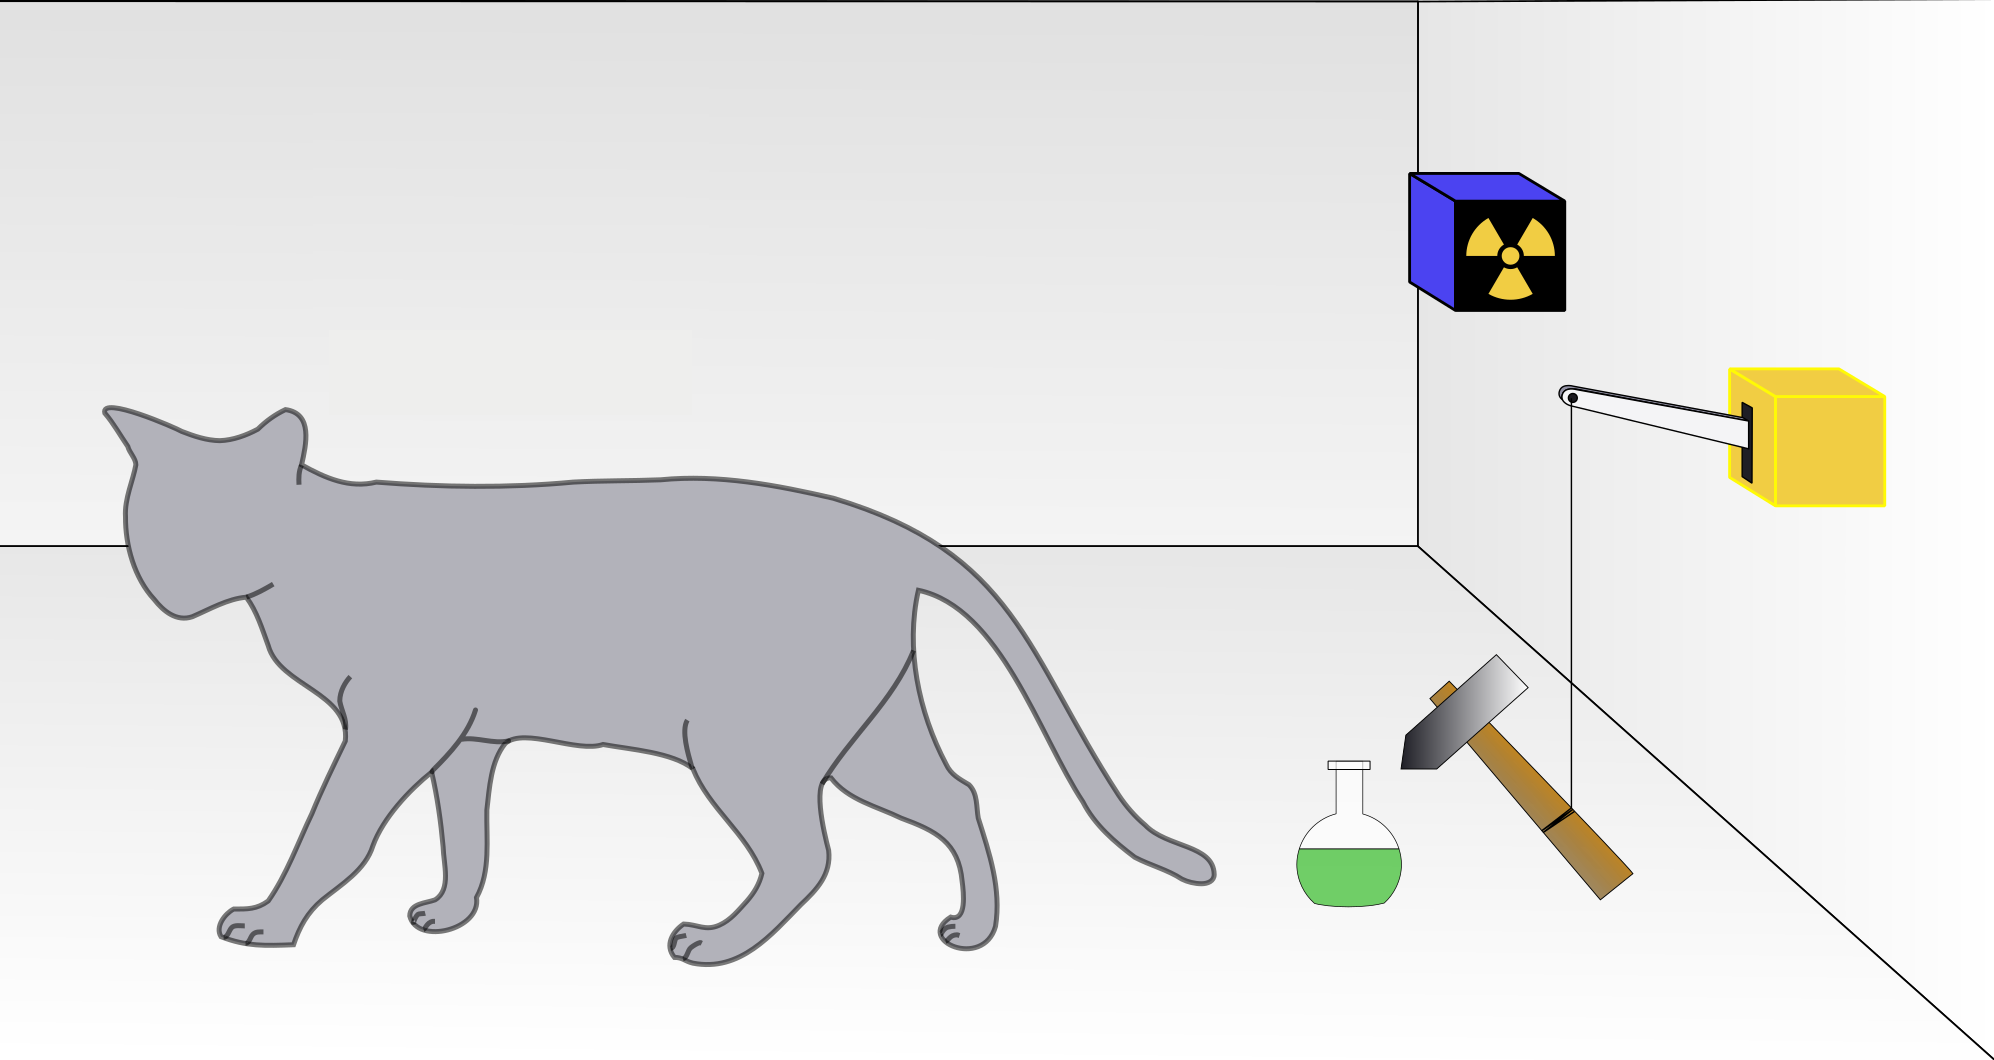
\includegraphics[width=100mm]{Chapter03/Schrodingers_livecat.png}
  \caption[Depiction of Schr\"{o}dinger's living cat]{A depiction of Schr\"{o}dinger's cat being alive.\protect\footnotemark}
  \label{livecat}
  \end{figure}
  \footnotetext{ Original by Dhatfield. This image is licensed under the Creative Commons Attribution-Share Alike 3.0 Unported license. Source: https://upload.wikimedia.org/wikipedia/commons/archive/9/91/20080627113554!Schrodingers\_cat.svg}

  \begin{figure}[ht!]
    \captionsetup{justification=justified}
    \centering
    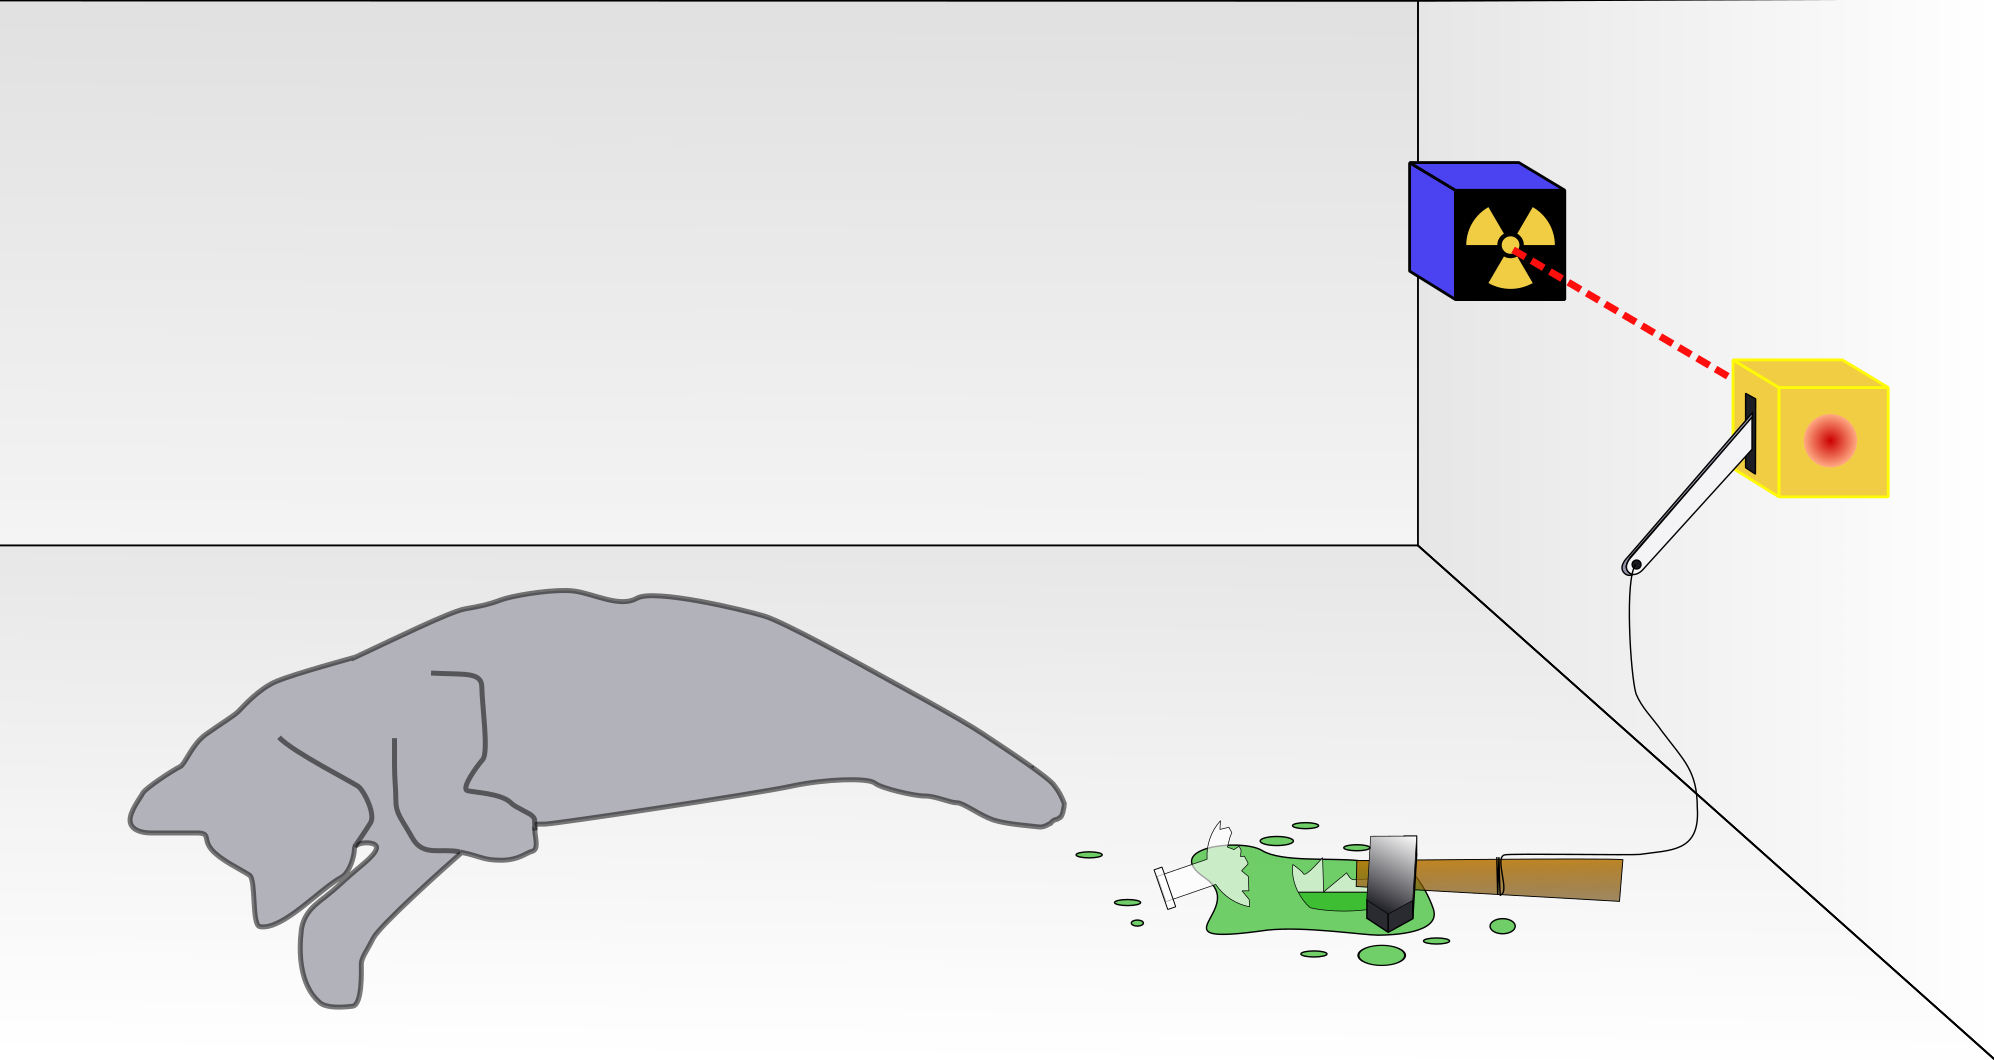
\includegraphics[width=100mm]{Chapter03/Schrodingers_deadcat.png}
    \caption[Depiction of Schr\"{o}dinger's dead cat]{A depiction of Schr\"{o}dinger's cat being dead.\protect\footnotemark}
    \label{deadcat}
    \end{figure}
\footnotetext{ Original by Dhatfield. Altered by removing numbers and making into two separate figures. This image is licensed under the Creative Commons Attribution-Share Alike 3.0 Unported license. Source: https://upload.wikimedia.org/wikipedia/commons/archive/9/91/20080627113554!Schrodingers\_cat.svg} 
    
One obvious objection to the above explanation is that one could imagine that the cat is in a box with perfectly mirrored walls, so that light from the cat can't escape. In such a situation, there would be no information about the cat's death or survival outside the relevant light cone, and so the cat would remain in a superposition of alive and dead states. Although perfectly mirrored walls are practically impossible, it would still seem rather problematic that the cat's having a well-defined life/death state depends on how perfectly reflective the walls of the box are. 

In responding to this objection, we should clarify that it is not necessary that light that has reflected directly off the cat must eventually intersect $S$ in order for the cat's state to be determined. Rather it is only necessary that light that has reflected off something that the cat is entangled with eventually intersects $S$. Now when light from the cat is reflected by the walls, the atoms in the walls affected by the light from the cat will get entangled with the cat, and the affected atoms will then interact with neighboring atoms which in turn will get entangled with the atoms that are entangled with the cat, and this entanglement will propagate through to the walls of the box, and when the light that reflects off the outside walls of the box is measured on $S$, this will contain some information about the state of the atoms of the outside walls and hence the atoms they are entangled with, and so this will ultimately lead to information about the state of the cat. 
    
One might still worry that it would still take a very long time for the light measured on $S$ to be sufficient to distinguish between the cat being alive and the cat being dead. We do however, have reason to think that this process might be very quick. For example, as already mentioned on page \pageref{electronspread},  if a free electron is initially described by a wave packet whose width is around $\du{e-10}{\m}$, then according to the Schr\"{o}dinger equation, after one second the width of the wave packet will have spread to a width of around $\du{1000}{\km}$. In reality, however, the electron remains relatively localized because of the scattering of light from the electron, and the light contains information that is able to localize the electron's position. So in the case of the cat in a box, the light reflecting off the outside of the box is at least going to contain enough information in the space of a second to determine that the cat is in the box rather than $\du{1000}{\km}$ away. And given that a cat is significantly larger than an electron, it seems very plausible that the light reflected off the outside of the box is going to contain significantly more information than the mere fact that the cat is in the box, and so we can reasonably expect there to be enough information in a short space of time to determine whether the cat is alive or dead.
    
    
\label{selectionmeaning} Another objection one could raise against Kent's interpretation is that it depends on the selection of a particular measurement outcome $\tau_S$ for the mass-energy density $T_S$ on $S$. However, Kent is rather vague about what he means by selection. Here is a (slightly edited) passage from Kent's 2014 paper that could do with some clarification:
\begin{adjustwidth}{1cm}{}
	\begin{displayquote}
    For any given hypersurface $S$ in the future of the initial hypersurface $S_0$, we consider the effect of joint measurements of the local mass-energy density $T_S(x)$ \ldots carried out at each point $x\in S$ \ldots. This gives us a probability distribution on possible mass-energy distributions $\tau_S(x)$ on $S$. In a universe in which physics starts on $S_0$ and ends on $S$, our picture of reality is that one $\tau_S(x)$ is randomly selected from the Born rule probability distribution. In other words, there is a randomly selected final boundary condition on S, which is defined mathematically in the same way that it would be if $T_S(x)$ were actually measured on S. However, we treat this simply as a mathematical algorithm. We do not suppose that a physical measurement actually takes place on $S$, or anywhere else. Our aim, instead, is to give a mathematical description of reality applicable to closed quantum systems, for which there are no external observers able to carry out measurements. To give a description of reality between $S_0$ and $S$, we use the initial state on $S_0$, the randomly chosen final outcome data $\tau_S(x)$ on $S$, and the unitary evolution law arising from the quantum dynamics.\footnote{\cite[2]{Kent2014}}
  \end{displayquote}
\end{adjustwidth}  
Now this passage raises two questions. Firstly, there is the question of what it means for the final outcome data $\tau_S$ on $S$ to be \emph{selected}, and secondly, there is the question of what it means for the final outcome data $\tau_S$ on $S$ to be selected \emph{randomly from the Born rule probability distribution}. 

With regard to the question of what it means to be selected, some greater clarity would be desirable since there will be other possible outcomes each of which will also have data describing them. It would therefore be helpful to know what we mean by predicating `selected' of one possible set of outcome data $\tau_S$, and predicating `not selected' of another set of outcome data $\tau_S'$? Now one suggestion would be to say that the predicate `selected' just means the attribution of some kind of quality $Q_\text{selected}$ to the outcome data $\tau_S$ which the outcome data $\tau_S'$ lacks. However, if we took this suggestion seriously, it would not be obvious why the quality $Q_\text{selected}$ of $\tau_S$ is a reason to consider the universe $\mathcal{U}$  whose description between $S_0$ and $S$ depended on $\tau_S$ was any more real than  the universe $\mathcal{U}'$  whose description between $S_0$ and $S$ depended on $\tau_S'$. In this case, we might therefore doubt that Kent was really proposing a one-world interpretation of quantum physics. 


A better way to think of what was meant by predicating `selected' of $\tau_S$ would be to say that it just means that $\tau_S$ is a property of $S$, namely at each $x\in S$, the mass-energy density $T_S(x)$ is given by $\tau_S(x)$. Such an understanding of $\tau_S$ being selected would then be no more problematic than predicating properties of a subject. And since $\tau_S'$ is not a property of $S$, we would not be inclined to think that a universe $\mathcal{U}'$  whose description between $S_0$ and $S$ depended on $\tau_S'$ was real. 

With regard to the question of what it means for $\tau_S$ to be randomly selected from the Born rule probability distribution, if there is only one state $\ket*{\Psi}$ such that $\hat{T}_S(x)\ket*{\Psi}=\tau_S(x)\ket*{\Psi}$ for all $x\in S$, then the probability $P(\tau_S)$ that $\tau_S$ is selected will be precisely the probability given by equation (\ref{bornpsi}). But if there are several states $\{\ket*{\Psi_\alpha}:\alpha\}$ such that  $\hat{T}_S(x)\ket*{\Psi_\alpha}=\tau_S(x)\ket*{\Psi_\alpha}$, then the probability $P(\tau_S)$ that $\tau_S$ is selected will be 
$$P(\tau_S)=\sum_\alpha \abs{\mel{\Psi_\alpha}{U_{SS_0}}{\Psi_0}}^2=\sum_\alpha \abs{\ip{\Psi_\alpha}{\Psi_S}}^2$$ 
where $\ket*{\Psi_S}=U_{SS_0}\ket*{\Psi_0}$. However, although we can state the Born rule probability $P(\tau_S)$ for $\tau_S$ to be selected, this doesn't tell us what it \emph{means} for $\tau_S$ to be selected with this probability. Given that Kent is proposing a one-world interpretation, he is presumably not thinking of this probability in frequentist terms as though there were many worlds with a certain proportion of them having the mass-energy density $T_S$ being given by $\tau_S$. One could try to understand the probability $P(\tau_S)$ as making a counter-factual claim: if there were many worlds, then a certain proportion of them would have the mass-energy density $T_S$ being given by $\tau_S$. But such a counter-factual claim seems irrelevant to the manner in which $\tau_S$ is selected. If $\tau_S'$ was another possible mass-energy density such that $P(\tau_S)\ll P(\tau_S')$,  then despite this inequality, $\tau_S$ could still be selected so long as $P(\tau_S)>0$, and so in this case, to say $\tau_S$ was selected with probability $P(\tau_S)$ is not obviously saying anything more than  $\tau_S$ was selected.

Perhaps we could instead think of the probability $P(\tau_S)$ in Bayesian terms, that is, maybe we should think of $P(\tau_S)$ as expressing a degree of belief that $\tau_S$ is the mass-energy density $T_S$. But again there is the problem of relevance: what relevance is my degree of belief to the fact that $\tau_S$ is selected? Perhaps I will be extremely surprised to learn that $\tau_S$ is selected, but my surprise doesn't make any difference to the fact that $\tau_S$ is selected. From a Bayesian perspective, there is also the further problem that there is going to be so much information in $\tau_S(x)$, and $P(\tau_S)$ is going to be so small due to the vast number of possible values for $T_S$, and so what is being claimed about $\tau_S$ when saying it has a probability $P(\tau_S)$ would be beyond the comprehension of any human mind to form any definite beliefs. 

Another alternative for what it means for $\tau_S$ to be randomly selected from the Born rule probability distribution $P(\tau_S)$ would be to say there is some threshold $\epsilon>0$ such that if $P(\tau_S)\geq\epsilon$, then $\tau_S$ is a possible value for $T_S$, whereas if $P(\tau_S)<\epsilon$, then  $\tau_S$ is not a possible value for $T_S$. Presumably, we could make $\epsilon$ sufficiently large so as to avoid scenarios in which there were stress-energy tensor values in regions between  $S_0$ and $S$ which corresponded to a cat being both dead and alive. Perhaps making $\epsilon$ larger still would ensure that a world whose description depended on $\tau_S$ with  $P(\tau_S)>\epsilon$ and in which there were sufficiently intelligent scientists would be a world in which scientists could formulate the theory of quantum physics as we know it based on their experimental observations. However, one problem with this suggestion is that the smaller $\epsilon$ is, the less the Born rule has any bearing on which $\tau_S$ is selected. If we permitted $\epsilon=0$, then the Born rule would have no relevance at all. Also, it would seem strange to treat the selection of two possible mass-energy densities $\tau_S$ and $\tau_S'$ in exactly the same way if $P(\tau_S)\gg P(\tau_S')>\epsilon$. 

Another way of thinking about the probability $P(\tau_S)$ would be to take the metaphor of God throwing dice: God throws some dice many times, and based on the sum of the outcomes, He chooses one of the $\tau_S$ in such a way that more probable sums correspond to $T_S$ outcomes with greater Born rule probability. Given such a scenario, we would need to explain the association between dice throws and $T_S$ outcomes -- perhaps God has a huge library of books each of which specifies a different $T_S$-outcome, and that when God  has summed up all His dice throws, He selects the book that has the same catalog number as this sum. Then finally, God makes $S$ have the same $T_S$ value as specified in the book He selected. However, one reason for having misgivings about such a suggestion is that we might think that each of the books that was not selected could still be considered to be just as real as the world described by the book that God did select. Therefore, if Kent's interpretation required something analogous to these books to make sense of the Born rule probability, we might worry whether his interpretation  really was a one-world interpretation of quantum physics. 

But perhaps another way of associating dice throws with $T_S$ outcomes would be to suppose that God lays a mesh over $S$ and determines the mass-energy density of each cell of the mesh in turn by using the following strategy: He first selects one of the cells whose mass-energy density He hasn't already determined; He then rolls some dice, and He then uses an algorithm to calculate the mass-energy density of the cell He has just selected where the algorithm depends on the dice outcome, the cell location, the initial state $\ket*{\Psi_0}$ of $S_0$, the mass-energy densities of the other cells He has previously determined, and a suitable application of the Born rule. Having determined the mass-energy density of this cell, God then selects another cell and uses the same strategy again to determine its mass-energy density, and so on until the mass-density $T_S$ is determined over the whole of $S$. There could be any number of variants of this strategy. For example, instead of saying that God directly causes all the cells of $S$ to have the mass-energy densities they have, maybe there are many beings each of which is assigned a particular region of $S$ whose mass-energy density the corresponding being is responsible for determining. Also, it is not obvious that randomness is essential ingredient in the selection of $T_S$. For example, instead of throwing dice, perhaps the digits of $\pi$ could be used in the determination of $T_S$, or maybe there are teleological principles at play in the history corresponding to the selected $T_S$ outcome $\tau_S$, even though it looks like $\tau_S$ could have been determined by a random process. 

Given the above discussion, it seems that the manner in which $T_S$ is selected is something we could speculate about endlessly. Kent assumes that the outcome of the notional measurement $T_S$ occurs with a probability given by the Born rule. However, it is not at all obvious what Kent means by this. Nevertheless, this lack of clarity is not necessarily a problem for Kent's interpretation. Rather, it just means that when it comes to selecting $T_S$, Kent's interpretation can accommodate a variety of philosophical preferences. But one would hope that given a particular $T_S$ outcome $\tau_S$, the history conditioned on $\tau_S$ would be one in which any scientists who performed measurements (in the normal sense of measurement) would measure average values of physical quantities consistent with the expectation values predicted by standard quantum theory. This intuition will be discussed in more detail in section \ref{KentconsistentQT}.




